\documentclass[../summary.tex]{subfiles}

\begin{document}
	
	\section{Mobility}
	
	\subsection{Study guide}
	
	This Chapter on mobility will be on the impact of person and freight transport and sustainable transport solutions. Make sure you:
	\begin{itemize}
	\item Understand the different strategies mentioned in this module (e.g. Mobility as a Service, Consolidation of freight transport,…)
	\item Understand the 4S framework and classify strategies for person and freight mobility according to this framework
	\item Understand the role price incentives (money) and technology can play to make our mobility pattern more sustainable
	\item Understand the links with the other modules
	\end{itemize}
	
	\subsection{Strategies}
	
	A first strategy to reduce the impact of our mobility systems, is a modal shift related to \textbf{cycling}. The more people we get on a bike, the better. An increased attention for the safety aspects and appropriate infrastructure is needed to encourage people to use a bike. More and more cities also implement a circulation plan. Such a plan explicitly steers the different traffic flows in and around a city, with one way streets and dead-end streets. It typically moves longer distance traffic around the city and limits the options for people with a destination inside the city. 
	\\\\
	Another important modal shift, is related to \textbf{public transport}. We want less cars on the road and more people using trains or buses. To have lower emissions per passenger-kilometer, we typically need around 10 people on a bus. To make public transport an attractive option, a good service is essential: comfortable, punctual and with a high frequency. Furthermore, the travel time using public transport should not be more than one-and-a-half time the travel time by car. That is why buses should not stop too often and can strongly benefit from separate bus lanes. But you also need to bring together the different flows and the different types of public transport in a network with a clear hierarchy. The large flows are served by a core network, with a high frequency, a high throughput and a high speed. For the smaller flows the service should be more flexible and “on-demand” to be effective and efficient. These on-demand services should bring people to the core network as efficient as possible.
	\\\\
	\textbf{Parcel delivery and small freight vans} are a large part of our current mobility challenges, and are expected to increase. A change in modal split can be initialized by local authorities: imposing limitations for trucks, limit the size of trucks that are allowed, using limited time windows in certain streets. Another option is called “consolidation”. The idea is that all parcels and freight are brought to the border of a city, for instance to a city hub. There, all these products are collected and then redistributed over smaller electric vehicles to be distributed in the city center in the most efficient way.
	\\\\
	\textbf{Mobility as a Service} combines different types of transport to ensure the wanted mobility. In this concept you are no longer the owner of your mode of transportation. This makes it easy and cheaper for the user to use more sustainable types of transport.
	
	\subsection{The 4S-framework}
	
	Today the demand for mobility of people and freight keeps growing. At the same time the available space is limited in and around most cities in the world. This combination leads to increasing congestion, loss of time and emissions. To deal with this challenge, there won't be a simple and straightforward solution, but we will require a combination of different steps. These steps can be divided in 4 categories: the \textbf{4S-framework}.
	\\\\
	The first category is \textbf{‘Suppress’}, this is about not having to make certain movement. A typical example here is working from home or having more online meetings.
	\\\\
	The second category is \textbf{‘Shorten’} or decrease the distance that you need to travel. For instance working closer to home or living closer to basic facilities like schools and shops.
	\\\\
	The third category is \textbf{‘Shift mode’}. A modal shift from car to bike or from truck to train. By using a different mode, we can often reduce traffic and/or environmental cost. For example, let’s take a look at the external environmental costs for freight transportation in Figure \ref{fig:external-environmental-costs}, calculated per 100 ton-kilometers. This graph sums up the costs of heavy metals, CO2, NOx, etc. Here we see a clear difference between for example trucks compared to trains.
	\\\\	
	The fourth category is \textbf{‘Smart technology’}. By improving the technology used in our vehicles, we can also reduce environmental cost. If we look at the same graph of Figure \ref{fig:external-environmental-costs}, we not only see a difference between the modes of transport, but we also see that the environmental cost has decreased between 2000 and 2014. This is due to technological improvements. 
	
	\begin{figure}[htbp]
		\centering
		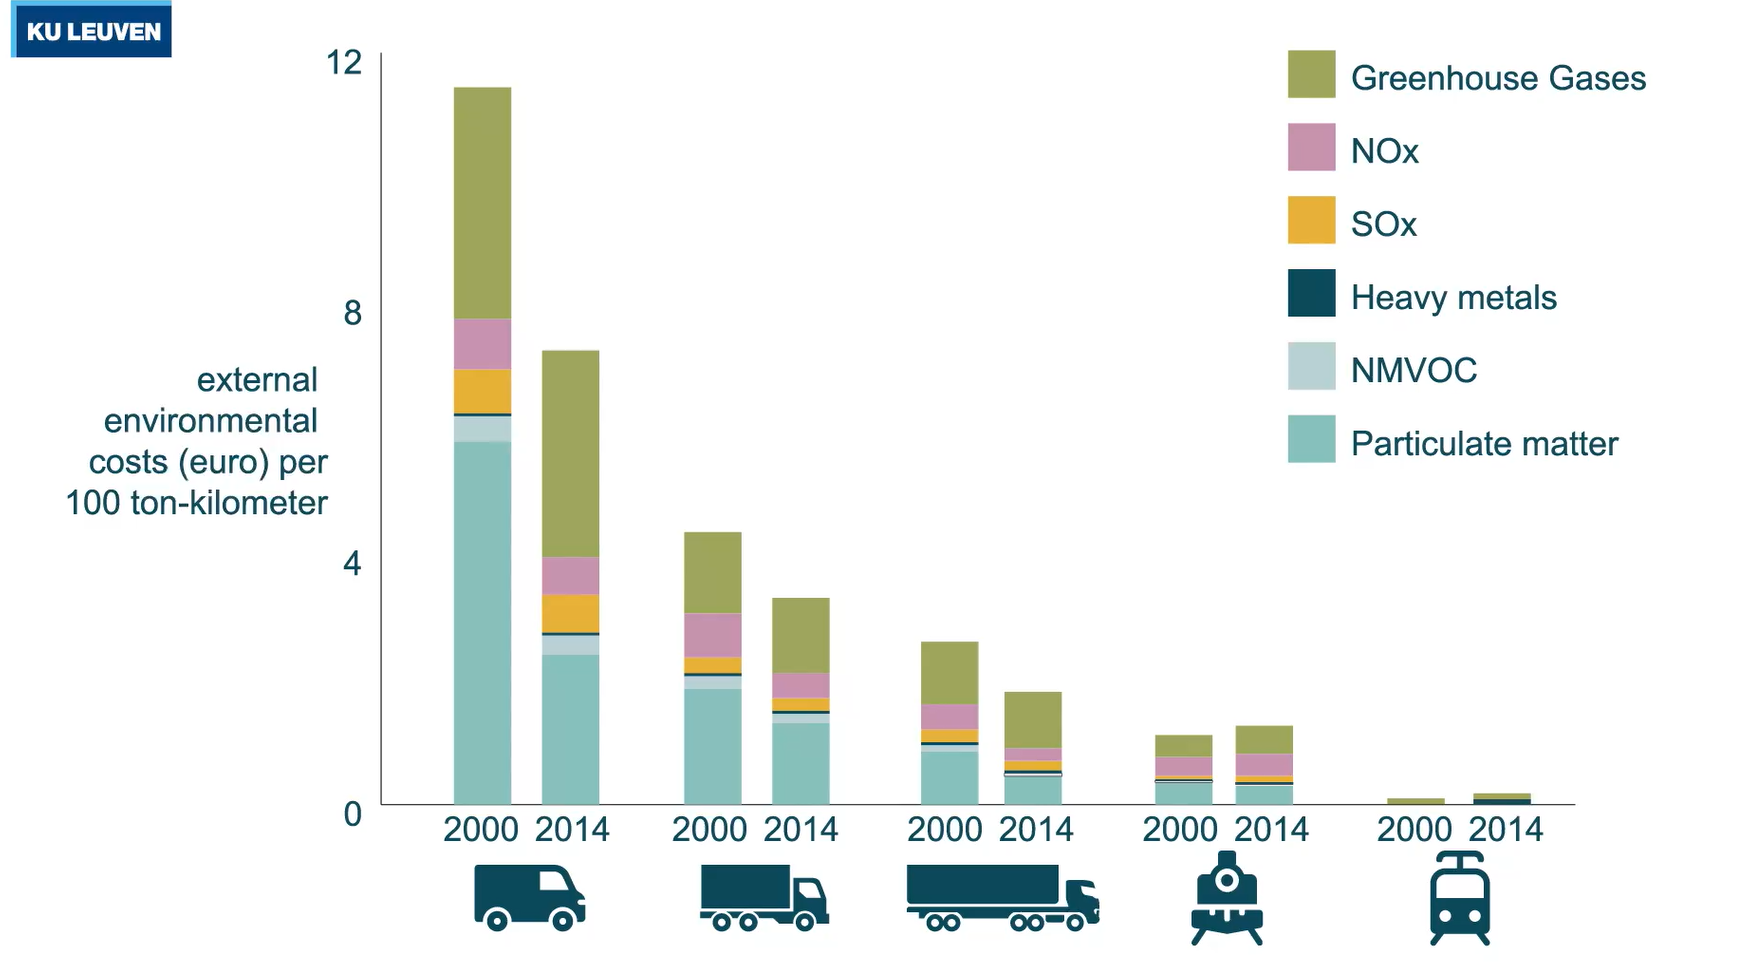
\includegraphics[width=1\linewidth]{images/9-external-environmental-cost.png}
		\caption{External environmental costs per 100 ton-kilometers, 2000 versus 2024}
		\label{fig:external-environmental-costs}
	\end{figure}
	
	\subsection{The role of price incentives and technology}
	
	When looking at the \textbf{financial aspect}, mobility is too often too cheap. The price of mobility should be increased, so mobility is considered more when decisions are taken. A first step in increasing the price, is by reducing systems that make transport cheaper, such as subsidized cars or free parcel delivery. There also needs to be an appropriate $CO_{2}$ pricing to discourage people from buying big cars that are often paired with increased emissions, an increase in fatal accidents with cyclists and pedestrians and other costs related to transport. 
	\\\\
	When the price of transport reflects the actual cost we will see four long term effects: People will live closer to their work. People will live closer together. People will work more from home. Parcel delivery and freight delivery will be bundled more. This solution is represented by the 4S-framework we discussed earlier. 
	\\\\
	Other \textbf{structural solutions} are related to infrastructure. \textbf{Low emission zones} clearly have a positive impact on emissions. They lead to greener cars and better air quality. \textbf{Circulation plans} with a clear choice for public transport, cycling and pedestrians also have a positive impact. 
	\\\\
	 Some people are convinced that \textbf{technological development} will solve all our problems, also all our mobility problems. An argument that is often  cited is the use of  \textbf{autonomous vehicles}. Clearly autonomous vehicles could have a large impact on both individual and public transport. It would probably be safer and cause less accidents. If some social hurdles were mitigated, it might also increase car - and ride sharing. It would seem that there are no downsides to autonomous vehicles. However, there is one problem: the switch to autonomous vehicles would be too late to prevent climate change. So, we need to find other solutions.
	 \\\\
	 One possible solution is \textbf{car sharing or other Uber-like systems}. This sounds good in theory because it decreased the number of vehicles. But in practice, it is currently just a cheap taxi-service, by poorly protected drivers, replacing movements by public transport or on foot. So, from a societal perspective many questions could and should be raised.
	 \\\\
	 Another possible solution in \textbf{hyperloop}. The basic idea is that you build tunnels underground or closed pipes above ground, and by making these almost vacuum, capsules or pods can travel through these pipes at enormous speeds, up to 1000km per hour. The believers promote the hyperloop for passengers by mentioning that it would not take up any space. However, this 'solution' brings problems related to its capacity. If you assume about 28 passengers per capsule, and a maximum frequency of 12 capsules per hour, giving you 5 minutes to put the capsule in the pipe, close the airlock and get it vacuum, then you get 336 passengers per hour per tube per direction. This is a lot less than the capacity of trains and planes that already exist. 
	 \\\\
	 To conclude, technological developments can play a part in solving the challenges related to mobility, but they should be properly managed and accompanied by more impactful measures, such as increasing the price of mobility.
	
	\subsection{Link with other modules}
	
	We can find multiple links with mobility and the other modules of this course. For instance, the is a link with \textbf{climate and biodiversity}. Transport accounts for around one-fifth of global CO2 emissions. About 75\% of these emissions comes from road vehicles for both passenger as freight transport. Apart from carbon, cars also emit NOx, SOx and particulate matter, leading not only to climate change but also to air pollution. 
	\\\\
	Another link that can be found is the one with \textbf{raw materials}. When addressing mobility related challenges, much is expected from the shift from current vehicles with combustion engines towards electric vehicles. It should be noted, however, that these electric vehicle also required the usage of raw materials, which are not always easily, and sustainably, available. 
	\\\\
	A third link we can find is a link with \textbf{economy and governance}. A worldwide or European CO2-tax would have a huge positive impact on climate change, certainly also related to mobility issues. A more detailed explanation on carbon taxing can be found in the module on Economy of sustainable development. 
	\\\\
	There also is a link with \textbf{energy}. Even after switching completely to electric vehicles instead of combustion engines, we still do not have a sustainable mobility system. Even then, for example, scarce raw materials and sustainable electricity generation are required.
	\\\\
	Last but not least, there also is a link between mobility and \textbf{inequality}. As mentioned in the module on inequality, many “sustainable” measures or solutions for the challenges require adjustments and special care to make them socially acceptable.
	
\end{document}